\documentclass[11pt]{article}
\usepackage[margin=1in]{geometry}
\usepackage{amsmath,amssymb}
\usepackage{booktabs}
\usepackage{array}
\usepackage{pdflscape}
\usepackage{graphicx}
\graphicspath{{../../figures/}}
\usepackage{hyperref}
\hypersetup{hidelinks}

\setlength{\parskip}{4pt plus 1pt minus 1pt}
\setlength{\parindent}{0pt}

\title{Genome as Projection:\\Coupling Channels Predict Cancer Survival\\and Suggest Drug Response Principles}
\author{Patrick D.\ McCarthy\\
\small Independent Researcher, Austin, TX\\
\small \texttt{pat.d.mccarthy@gmail.com}}
\date{}

\begin{document}
\maketitle

\begin{abstract}
The genome is a linear projection of a functional graph. Genes that
appear distinct in sequence can be copies of the same functional
node, forced into separate addresses by serialization. We call these
\textbf{projection families}. The distributed connectivity between
them, too diffuse to encode in any single gene, we call
\textbf{coupling channels}.

This reframing has three consequences. First, the number of coupling
channels a tumor disrupts predicts survival; the number of mutations
does not. We demonstrate this across 73{,}593 patients. Second,
genes in the same projection family carry the same drug
vulnerability. We predict expanded eligibility for PARP, PI3K/AKT,
and FGFR inhibitors, explain published combination failures, and
identify a timing principle for cross-channel therapy. Third,
channel severance by any mechanism produces the same cancer risk.
We predict specific patterns for transplant immunosuppression,
neurodegeneration, and information-environment exposure.

Screen by function, not by gene name.
\end{abstract}

% ------------------------------------------------------------------
\section{Introduction}
\label{sec:intro}
% ------------------------------------------------------------------

The functional relationships between genes form a dense, cyclic
graph. The genome is a linear sequence. Serializing one into the
other forces copies: a single genomic address cannot serve all
adjacencies of a hub node. Paralogs, gene families, ``functionally
related'' genes are projection artifacts. They are copies of the
same node at different addresses.

This paper makes three claims of decreasing certainty.

\textbf{Demonstrated: Channel count predicts survival.} Across
73{,}593 patients, the number of channels disrupted predicts overall
survival ($p < 10^{-44}$). Mutation count does not. More mutations
in fewer channels means deeper commitment to one escape route: a
more constrained, treatable tumor. Section~\ref{sec:empirical}.

\textbf{Interpretive: Channels are the distributed graph.} A
coupling channel is not a pathway. It is the organizational function
a pathway serves. Channels are the connectivity too distributed to
precipitate into any single gene. Section~\ref{sec:framework}.

\textbf{Predictive: The framework generates falsifiable predictions.}
If genes in the same family are copies of the same functional node,
they carry the same vulnerability. A drug that works on one should
work on all. If channels can be severed by any mechanism, non-genetic
channel disruption should produce predictable cancer risk patterns.
Section~\ref{sec:predictions} presents specific predictions spanning
drug response, graph topology, and non-genetic severance.

Paper~4 of this series \cite{McCarthy2026d} proves that bounded
active context determines an entity's capability: reducing context
reduces effective intelligence. This paper tests that prediction.
Cancer is escalation chain severance. Coupling channels connect
cells to tissue, organ, and organism levels. Severing them reduces
the cell's effective context, forcing cell-level optimization.
Channel count measures how much context is lost. Survival measures
how well the reduced entity persists. The formal derivations appear
in \cite{McCarthy2026a, McCarthy2026b, McCarthy2026c,
McCarthy2026d}. This paper can be read independently.

% ------------------------------------------------------------------
\section{Empirical Result: Channel Count Predicts Survival}
\label{sec:empirical}
% ------------------------------------------------------------------

We tested the central claim, that channel count predicts survival
better than mutation count, using three publicly available datasets
from cBioPortal \cite{Cerami2012}: the MSK-IMPACT Clinical
Sequencing Cohort ($n = 7{,}091$ patients, 2{,}126 deaths;
pan-cancer) \cite{Zehir2017}, the MSK MetTropism Cohort
($n = 24{,}646$ patients, 9{,}893 deaths; metastatic)
\cite{Nguyen2022}, and the MSK-IMPACT 50K Cohort
($n = 41{,}856$ patients, 16{,}731 deaths; pan-cancer)
\cite{Bandlamudi2024}. Together: 73{,}593 patients, 28{,}750 deaths.

\subsection{Method}

For each patient, we mapped somatic mutations to six coupling
channels based on the organizational function of the mutated gene:
(1)~DNA damage response (DDR: \emph{BRCA1}, \emph{BRCA2},
\emph{ATM}, \emph{CHEK2}, mismatch repair genes),
(2)~cell cycle checkpoint (\emph{TP53}, \emph{RB1}, \emph{CDKN2A},
\emph{CDK4/6}),
(3)~growth signaling (PI3K--AKT--mTOR, RAS--MAPK:
\emph{PIK3CA}, \emph{PTEN}, \emph{KRAS}, \emph{BRAF}, \emph{EGFR},
\emph{ERBB2}),
(4)~endocrine/hormone (\emph{ESR1}, \emph{GATA3}, \emph{FOXA1},
\emph{AR}),
(5)~immune surveillance (\emph{B2M}, \emph{HLA-A/B/C},
\emph{JAK1/2}),
(6)~tissue architecture (\emph{CDH1}, \emph{APC}, \emph{CTNNB1},
\emph{SMAD4}, \emph{NOTCH1}).
Non-silent mutations (missense, nonsense, frameshift, splice site)
in these genes. For each patient, we recorded the number of
\emph{distinct channels} with at least one mutation.
The channel mapping and analysis code are provided in the
supplementary repository.

\subsection{Results}

\textbf{Channel count predicts survival; mutation count does not.}
Table~\ref{tab:empirical} summarizes Cox proportional hazards
results across all three datasets. In multivariate models, channel
count is significant in every dataset ($p < 0.005$). Mutation count
either drops out (MSK-IMPACT 2017: $p = 0.67$) or becomes
\emph{protective} (MetTropism: HR $= 0.82$; 50K: HR $= 0.83$).
If channel count proxied for tumor burden, mutation count would
predict worse outcomes. It predicts better.

\begin{figure}[ht]
\centering
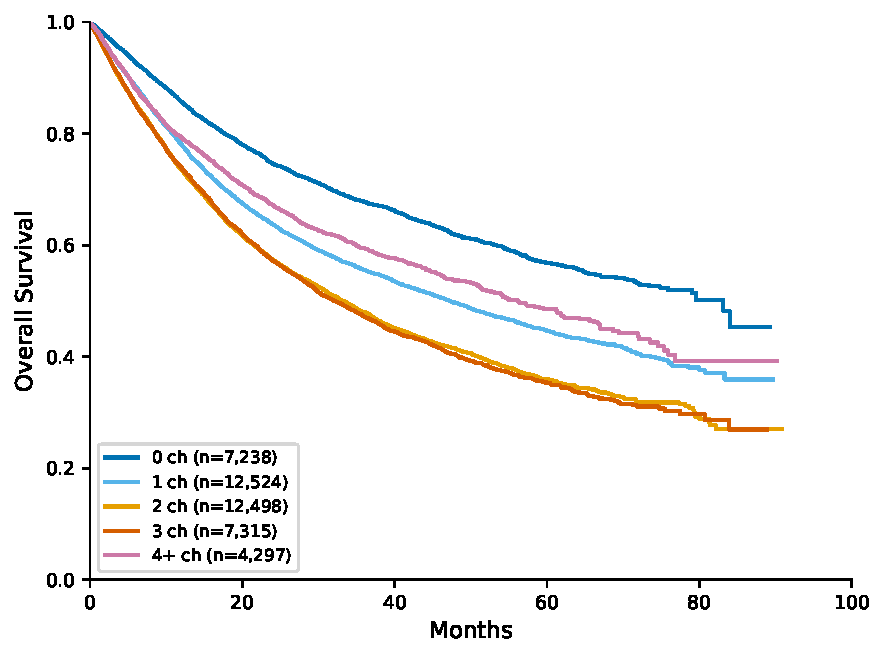
\includegraphics[width=0.85\textwidth]{km_by_channel_count.pdf}
\caption{Kaplan--Meier survival curves stratified by the number of
coupling channels severed (MSK-IMPACT 50K, $n = 43{,}872$;
Cox regression in Table~\ref{tab:empirical} uses $n = 41{,}856$
after excluding patients with missing covariates). Survival
decreases monotonically from 0 to 3 channels. The 4+ group shows
partial rebound, consistent with hypermutation phenotypes where
most mutations are passengers.}
\label{fig:km}
\end{figure}

\begin{table}[ht]
\centering
\caption{Cox proportional hazards: channel count vs.\ mutation
count across three independent cohorts totaling 73{,}593 patients.
HR\,$=$\,hazard ratio per unit increase (95\% CI).
In multivariate models,
channel count remains significant while mutation count loses
predictive power or becomes protective.}
\label{tab:empirical}
\medskip
\begin{tabular*}{\textwidth}{@{\extracolsep{\fill}}llccl@{}}
\toprule
Dataset & Predictor & HR (95\% CI) & $p$ & Note \\
\midrule
MSK-IMPACT 2017 & Channel count (univariate) & 1.10 & $<$0.005 & \\
\quad ($n=7{,}091$) & Log mutation count (univariate) & 1.12 & $<$0.005 & \\
 & Channel count (multivariate) & 1.09 & $<$0.005 & Significant \\
 & Log mutation count (multivariate) & 1.02 & 0.67 & Not significant \\
\midrule
MetTropism & Channel count (univariate) & 1.06 & $<$0.005 & \\
\quad ($n=24{,}646$) & Log mutation count (univariate) & 1.00 & 0.69 & Not significant \\
 & Channel count (multivariate) & 1.17 & $<$0.005 & Significant \\
 & Log mutation count (multivariate) & 0.82 & $<$0.005 & Protective \\
\midrule
MSK-IMPACT 50K & Channel count (univariate) & 1.04 & $<$0.005 & \\
\quad ($n=41{,}856$) & Log mutation count (univariate) & 0.98 & 0.03 & Weakly protective \\
 & Channel count (multivariate) & 1.15 & $<$0.005 & Significant \\
 & Log mutation count (multivariate) & 0.83 & $<$0.005 & Protective \\
\bottomrule
\end{tabular*}
\end{table}

\textbf{Cross-channel co-mutations are worse than same-channel.}
Two mutations in different channels produce worse outcomes than
two mutations in the same channel (Table~\ref{tab:cross-channel}).
Cross-channel patients have higher average mutation counts, but the
multivariate Cox model (Table~\ref{tab:empirical}) controls for
this: channel count is significant after adjusting for mutation
count.

Multi-region sequencing explains why. Gerlinger et~al.\
\cite{Gerlinger2012} showed that 63--69\% of somatic mutations in
renal cell carcinoma are not shared across tumor regions, and
different regions independently acquire mutations in the same
pathway through parallel evolution. The TRACERx consortium
\cite{JamalHanjani2017, Swanton2023} confirmed the pattern in
NSCLC: trunk mutations (clonal, present in every cancer cell) are
the initiating channel break; branch mutations (subclonal,
region-specific) are later hits, with parallel evolution recurring
in RAS, PIK3CA, SWI/SNF, and immune evasion genes.

The mechanism is channel-level synthetic lethality. Two channel
breaks in the same cell are lethal: the cell loses two independent
defense systems and cannot sustain viability. A patient with
channel count~$= 2$ does not have one clone with two breaks. The
patient has two clonal populations, each with a single channel
break. The patient-level mutation profile is an aggregate across
heterogeneous subclones. Channel count therefore measures clonal
diversity: more channels severed means more independently viable
lineages, each exploiting a different defense vulnerability.

This explains three otherwise puzzling results. First, why
cross-channel is worse than same-channel: two mutations in the
same channel can coexist in one cell (within-channel redundancy),
but two mutations in different channels cannot, so cross-channel
patients necessarily harbor more heterogeneous tumors. Second, why
same-channel depth is protective: deeper commitment to one channel
means a more clonally homogeneous tumor, presenting a single
therapeutic target. Third, why mutation count becomes protective
after controlling for channel count: additional mutations within an
already-severed channel do not generate new clonal lineages.

\begin{table}[ht]
\centering
\small
\caption{Cross-channel vs.\ same-channel co-mutation mortality.
Cross-channel: 2+ mutations hitting different coupling channels.
Same-channel: 2+ mutations confined to one channel. The difference
is significant in all three datasets.}
\label{tab:cross-channel}
\begin{tabular}{@{}lrrrl@{}}
\toprule
Dataset & Cross-channel & Same-channel & $p$ (log-rank) \\
\midrule
MSK-IMPACT 2017 ($n=7{,}091$) & 33.1\% & 27.7\% &
  $1.4 \times 10^{-5}$ \\
MetTropism ($n=24{,}646$) & 42.9\% & 39.0\% &
  $6.3 \times 10^{-13}$ \\
MSK-IMPACT 50K ($n=41{,}856$) & 42.6\% & 39.7\% &
  $5.7 \times 10^{-13}$ \\
\bottomrule
\end{tabular}
\end{table}

\textbf{Synthetic lethality is tissue-conditional.}
Known synthetic lethal (SL) gene pairs show mutual exclusivity in
tumors: cells that lose both copies of a functional node die, so
double knockouts are absent from patient data. If SL partners are
copies of the same functional node at different genomic addresses,
the exclusivity should depend on whether the channel those genes
serve is load-bearing in that tissue.

Figure~\ref{fig:sl-by-ct} shows the obs/exp ratio for 121 SL gene
pairs across 41 cancer types ($n = 44{,}283$). The variation is
fivefold. Ovarian cancer (obs/exp $= 0.74$), NSCLC (0.76), and
squamous lung (0.87) show strong mutual exclusivity. These are the
cancer types where PARP inhibitors have demonstrated clinical
efficacy. Colorectal (2.60) and endometrial (2.97) show strong
co-occurrence. Both are MSI-high cancers: mismatch repair is already
gone, the DDR array has already failed, and the exclusivity
constraint relaxes. The co-mutation matrix alone, without survival
data, maps which channels are load-bearing in which tissues.

\begin{figure}[ht]
\centering
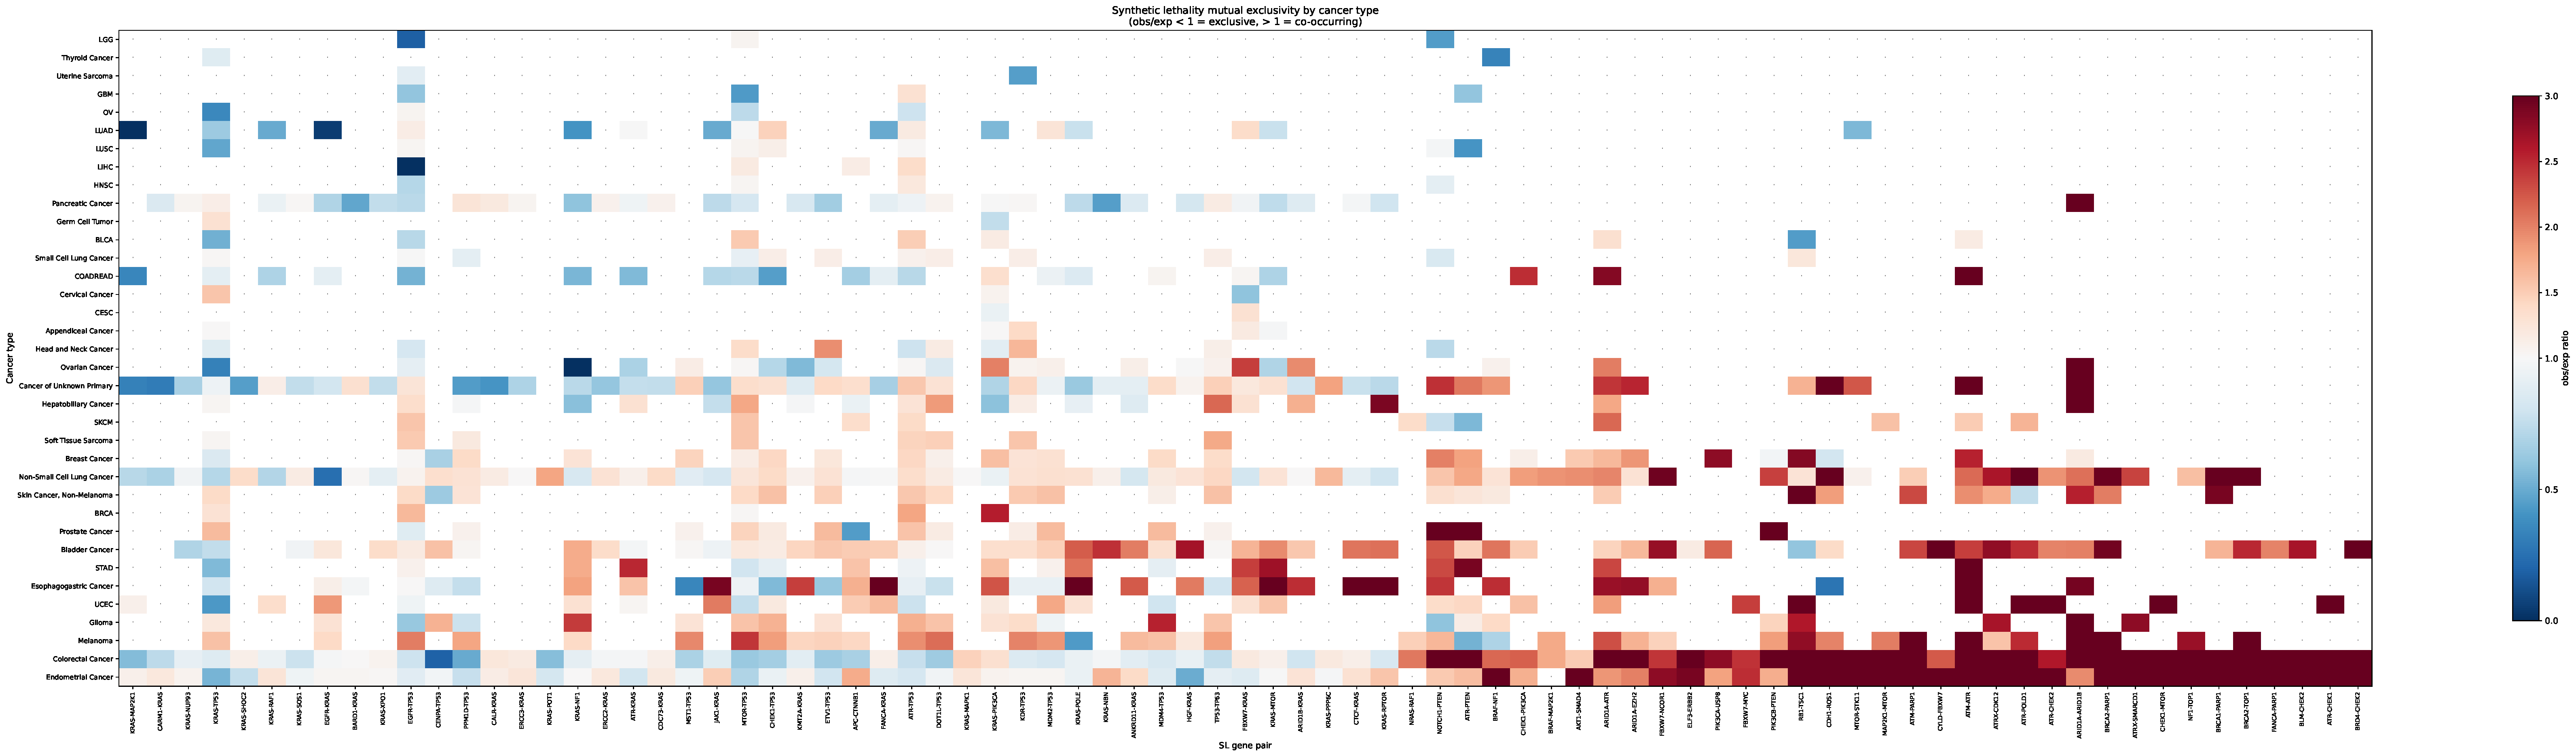
\includegraphics[width=0.95\textwidth]{sl_exclusivity_by_ct.pdf}
\caption{Synthetic lethality mutual exclusivity by cancer type.
Each cell shows the observed/expected co-mutation ratio for an SL
gene pair in a given cancer type. Blue (obs/exp $< 1$): mutually
exclusive, the channel is load-bearing. Red (obs/exp $> 1$):
co-occurring, the channel is bypassed or the tumor is hypermutated.
Cancer types are sorted by mean exclusivity. The pattern predicts
where PARP inhibitors should be effective (blue rows) and where they
should not (red rows).}
\label{fig:sl-by-ct}
\end{figure}

\textbf{Same-channel depth: more mutations in fewer channels is
protective.} Stratifying by fixed channel count, patients with more
mutations survive longer. At 2 channels: mortality drops from 46.2\%
to 41.2\% ($p = 3.1 \times 10^{-8}$). At 3 channels: 46.9\% to
38.6\% ($p = 7.2 \times 10^{-14}$). MetTropism replicates: at
3 channels, 49.6\% vs.\ 36.5\% ($p = 2.6 \times 10^{-10}$).

An alternative explanation is immunogenicity: more mutations produce
more neoantigens and better immune response. If neoantigen load
explained the protective effect, it should also protect
cross-channel patients. It does not (Table~\ref{tab:cross-channel}).
The protection is specific to same-channel depth, not total mutation
burden.

\textbf{Mortality gradient by channel count.} All three datasets
show a monotonic mortality gradient from 0 to 3--4 channels
severed (Figure~\ref{fig:km}). In the 50K cohort: 30.4\% (0~channels), 38.5\% (1),
44.2\% (2), 44.3\% (3), 40.3\% (4). Patients with 5--6 channels
show lower mortality (29.0\%, 20.7\%), consistent with the
hypermutation phenotype (MSI-high, mismatch repair deficient) where
most mutations are passengers that do not functionally sever channels.

\textbf{Sensitivity to channel granularity.} The six-channel mapping
is one hypothesis. To test robustness, we repeated the multivariate
Cox regression at every granularity from 2 to 10 channels.
Table~\ref{tab:sensitivity} shows the results for the MSK-IMPACT
50K cohort (the two smaller datasets replicate the same pattern).

\begin{table}[ht]
\centering
\caption{Sensitivity analysis (MSK-IMPACT 50K, $n = 41{,}856$):
multivariate Cox hazard ratios for channel count and log mutation
count at different channel granularities. Channel count is
significant from 2 through 8 channels, peaks at 3, and collapses
at 10. All three datasets replicate this pattern.}
\label{tab:sensitivity}
\medskip
\begin{tabular*}{\textwidth}{@{\extracolsep{\fill}}rcccc@{}}
\toprule
Channels & Ch HR & Ch $p$ & Mut HR & Mut $p$ \\
\midrule
2 & 1.25 & $2 \times 10^{-52}$ & 0.94 & $4 \times 10^{-9}$ \\
3 & 1.30 & $3 \times 10^{-124}$ & 0.86 & $8 \times 10^{-41}$ \\
4 & 1.21 & $3 \times 10^{-75}$ & 0.88 & $9 \times 10^{-27}$ \\
5 & 1.17 & $8 \times 10^{-58}$ & 0.88 & $6 \times 10^{-22}$ \\
6 & 1.14 & $1 \times 10^{-44}$ & 0.90 & $2 \times 10^{-16}$ \\
7 & 1.10 & $7 \times 10^{-24}$ & 0.93 & $1 \times 10^{-7}$ \\
8 & 1.07 & $3 \times 10^{-14}$ & 0.95 & $4 \times 10^{-4}$ \\
10 & 1.01 & 0.064 & 1.02 & 0.20 \\
\bottomrule
\end{tabular*}
\end{table}

The signal peaks at 3 channels ($p = 3 \times 10^{-124}$) and is
significant from 2 through 8. At 10, over-splitting collapses
channel count back into a proxy for mutation count. The specific
number matters less than the principle: grouping by organizational
function outpredicts counting mutations at every reasonable
granularity.

\textbf{Cancer-type adjustment.} Adding cancer type as a covariate
(38 types, one-hot) attenuates channel count by 1.1\% in the 50K
cohort (HR~$= 1.17$, $p = 8 \times 10^{-73}$). MetTropism: 16\%
attenuation, still significant ($p = 2 \times 10^{-47}$).
Within-type analysis confirms: NSCLC (HR~$= 1.16$),
breast (HR~$= 1.29$), prostate (HR~$= 1.47$),
pancreatic (HR~$= 1.32$), all $p < 10^{-10}$.
Channel count is not a proxy for cancer type.
Figure~\ref{fig:channel-by-ct} shows the channel severance
frequency for each cancer type. The pattern is tissue-specific:
breast cancer is dominated by PI3K/Growth and Endocrine; glioma by
Cell Cycle and DDR; colorectal by Tissue Architecture and
PI3K/Growth. Channels reflect organizational dependencies, not
statistical artifacts.

\begin{figure}[ht]
\centering
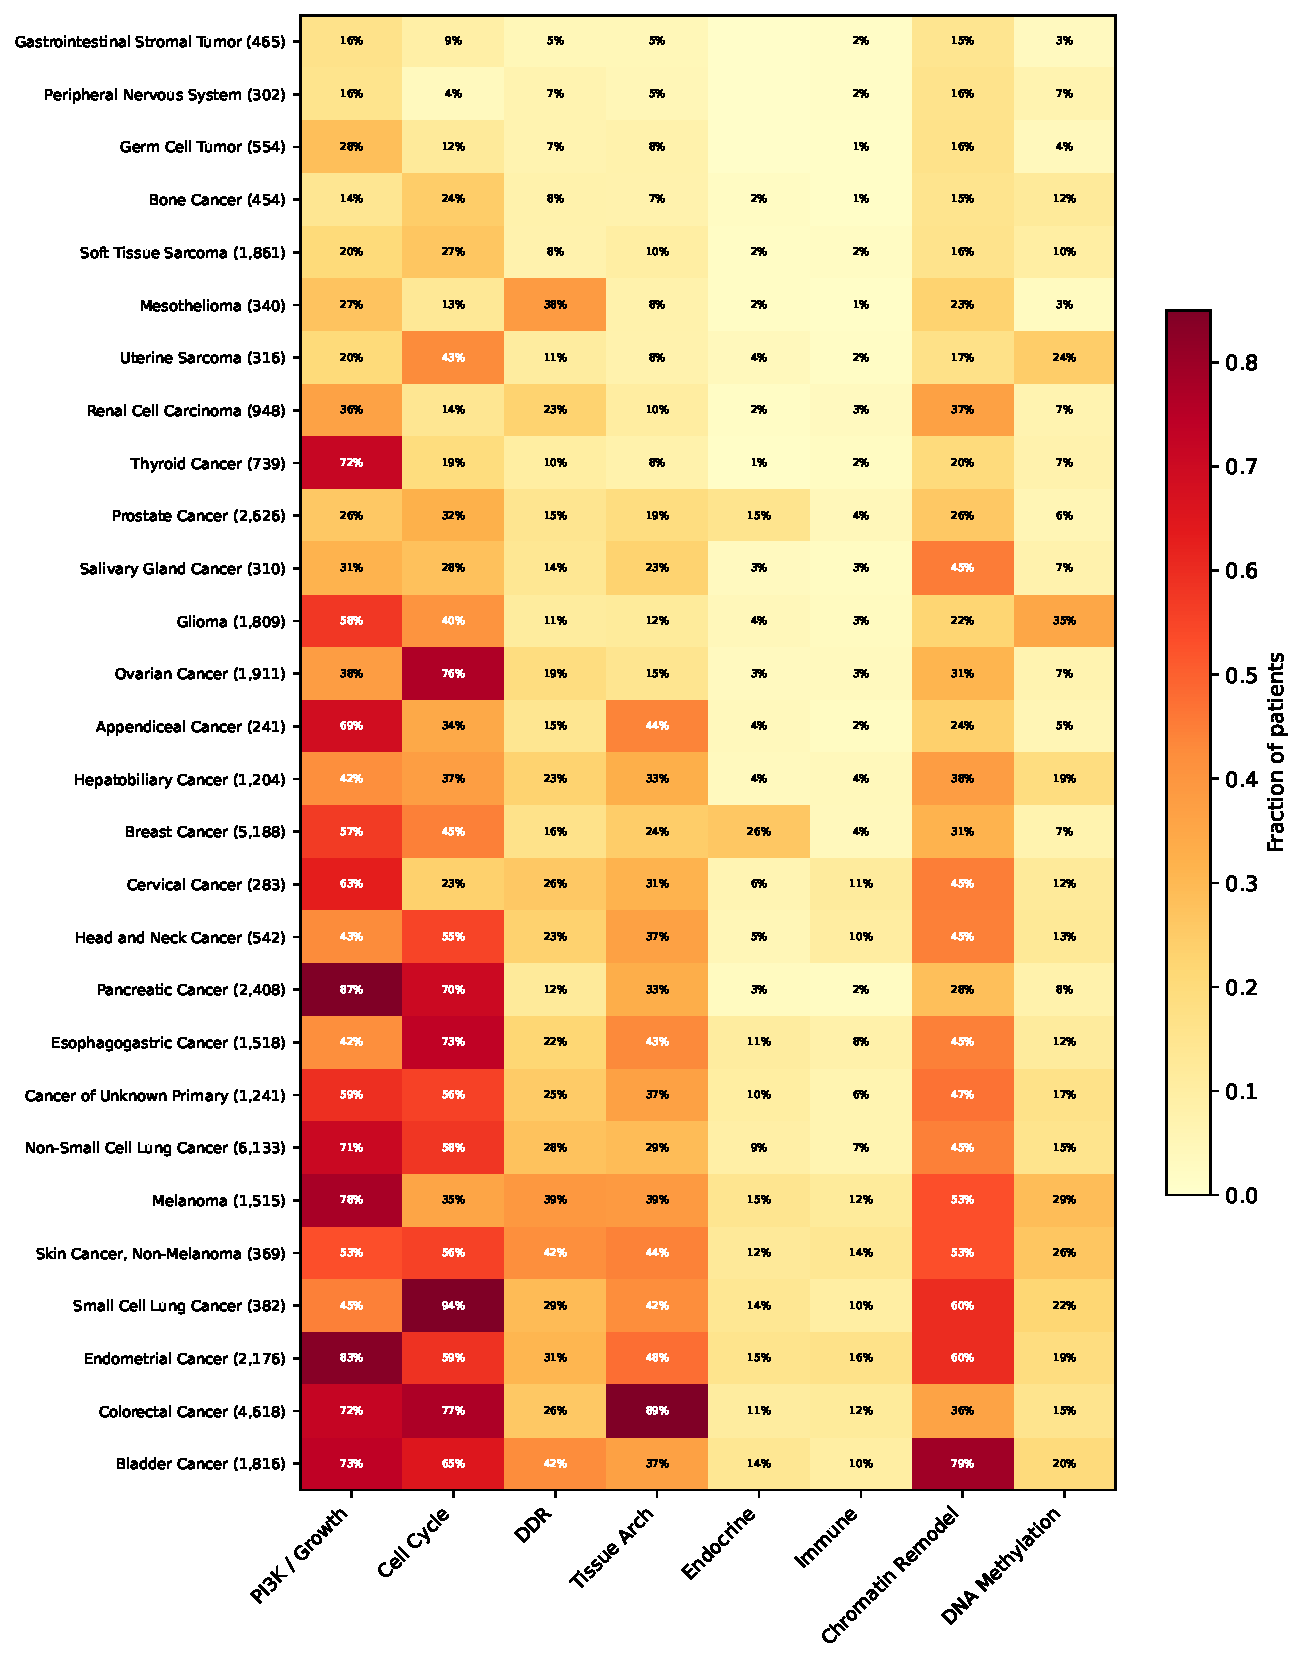
\includegraphics[width=0.95\textwidth,height=0.85\textheight,keepaspectratio]{channel_frequency_by_ct.pdf}
\caption{Channel severance frequency by cancer type. Each cell
shows the fraction of patients in that cancer type with at least one
mutation in the given channel. Cancer types are sorted by total
channel burden. The tissue-specific pattern confirms that channels
reflect organizational dependencies: breast is Endocrine-dominant,
colorectal is Tissue Architecture-dominant, glioma is Cell
Cycle-dominant.}
\label{fig:channel-by-ct}
\end{figure}

\textbf{Channel identity vs.\ gene degree per cancer type.}
Network degree---the number of protein interactions a gene
participates in---predicts survival pan-cancer ($p = 10^{-39}$).
But per-cancer-type analysis reveals that degree is significant in
only 15 of 29 evaluable cancer types, while channel identity
(which of the six channels is mutated) is significant in 22 of 29
(Table~\ref{tab:degree-vs-channel}).
Degree is a roll-up: it measures whether TP53 or CDKN2A is mutated.
Channel identity captures which organizational function failed.
In seven cancer types---colorectal, glioma, esophagogastric,
melanoma, renal cell, small bowel, and small cell lung---degree is
non-significant while at least one channel reaches $p < 0.05$.
In colorectal cancer ($n = 4{,}596$), degree contributes nothing
($p = 0.36$), but PI3K/Growth ($p = 1.8 \times 10^{-8}$) and
Immune ($p = 8.5 \times 10^{-7}$) are highly significant.
In glioma ($n = 1{,}457$), degree is marginal ($p = 0.08$)
while PI3K/Growth alone reaches $p = 5.9 \times 10^{-18}$.

\begin{table}[ht]
\centering
\caption{Channel identity vs.\ network degree, per cancer type
(MSK-IMPACT 50K). Each row shows the best channel $p$-value from a
six-channel Cox model and the degree-only $p$-value for the same
cohort. 99 genes mapped to 6 channels across 468 panel genes.
Cancer types with $n < 100$ or $<30$ events excluded.}
\label{tab:degree-vs-channel}
\medskip
\small
\begin{tabular*}{\textwidth}{@{\extracolsep{\fill}}lrcccl@{}}
\toprule
Cancer Type & $n$ & Degree $p$ & Channel $p$ & \#sig & Best channel \\
\midrule
Breast                    & 4709 & $2 \times 10^{-30}$ & $2 \times 10^{-37}$ & 4 & CellCycle \\
Prostate                  & 1747 & $5 \times 10^{-14}$ & $3 \times 10^{-17}$ & 2 & CellCycle \\
Thyroid                   &  597 & $3 \times 10^{-16}$ & $5 \times 10^{-16}$ & 1 & CellCycle \\
Endometrial               & 2150 & $6 \times 10^{-20}$ & $1 \times 10^{-14}$ & 5 & CellCycle \\
Pancreatic                & 2227 & $1 \times 10^{-10}$ & $6 \times 10^{-6}$  & 2 & CellCycle \\
NSCLC                     & 5578 & $1 \times 10^{-9}$  & $3 \times 10^{-10}$ & 2 & CellCycle \\
\midrule
Colorectal                & 4596 & 0.36                & $2 \times 10^{-8}$  & 5 & PI3K\_Growth \\
Glioma                    & 1457 & 0.08                & $6 \times 10^{-18}$ & 1 & PI3K\_Growth \\
Melanoma                  & 1323 & 0.005               & $4 \times 10^{-5}$  & 3 & PI3K\_Growth \\
Esophagogastric           & 1422 & 0.78                & 0.068               & 0 & Endocrine \\
Renal Cell                &  568 & 0.25                & 0.022               & 1 & CellCycle \\
Small Bowel               &  129 & 0.27                & $2 \times 10^{-3}$  & 1 & Immune \\
Small Cell Lung           &  375 & 0.69                & 0.021               & 1 & PI3K\_Growth \\
\bottomrule
\end{tabular*}
\end{table}

The top block: both degree and channel are significant, with comparable
or stronger $p$-values for channels. The bottom block: degree is
non-significant, but the channel model identifies exactly which
organizational function is load-bearing in that tissue.
This is not a modeling improvement. It is a structural claim:
cancer is not ``high-degree gene mutated.'' Cancer is ``this
channel severed in this tissue.'' Degree absorbs that signal
pan-cancer because CellCycle genes (TP53, CDKN2A) are
high-degree. Per cancer type, the channel is the ground truth.

\textbf{Full covariate adjustment.} Kitchen-sink Cox model: TMB, MSI,
cancer type, subtype, age, sex, tumor purity, FGA, primary site,
sample type, panel version. 275 covariates in the 50K cohort.
Channel count: HR~$= 1.09$, $p = 10^{-23}$. MetTropism
(187 covariates): HR~$= 1.11$, $p = 10^{-18}$. MSK-IMPACT 2017
(109 covariates): HR~$= 1.14$, $p = 2 \times 10^{-8}$.

\textbf{Severance hierarchy: cell-intrinsic channels first.}
The six coupling channels are not severed at random
(Figure~\ref{fig:hierarchy}). Among patients
with exactly one channel severed ($n = 12{,}558$), 80\% have
PI3K/Growth Signaling or Cell Cycle: the cell-intrinsic channels
that govern proliferation. Endocrine and Immune account for fewer
than 5\%. Among patients with two or more channels severed
($n = 24{,}535$), 98.1\% have at least one cell-intrinsic channel.

The progression ladder is:
\begin{itemize}
\item \textbf{1~channel}: PI3K/Growth (44.5\%) or Cell Cycle
  (35.7\%) dominate. Immune: 0.7\%.
\item \textbf{2~channels}: PI3K/Growth rises to 73.9\%, Cell Cycle
  to 64.6\%. Tissue Architecture enters at 33.6\%.
\item \textbf{3~channels}: PI3K/Growth at 90.8\%, Cell Cycle 80.9\%,
  Tissue Architecture 70.8\%. Endocrine (13.5\%) and Immune (7.2\%)
  remain rare.
\item \textbf{4~channels}: PI3K/Growth at 96.7\%. Endocrine and
  Immune are the last additions (30\%, 25\%).
\end{itemize}

\begin{figure}[ht]
\centering
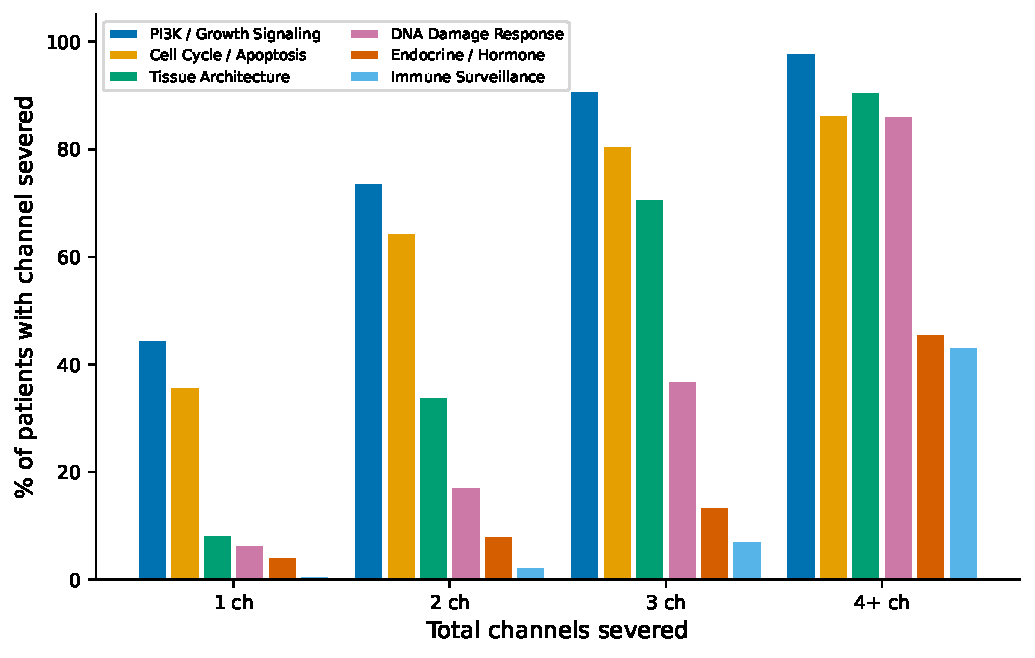
\includegraphics[width=0.9\textwidth]{severance_hierarchy.pdf}
\caption{Severance hierarchy across channel-count strata
(MSK-IMPACT 50K). Each bar shows the percentage of patients at a
given stratum who have that channel severed. Cell-intrinsic channels
(PI3K/Growth, Cell Cycle) dominate at every stratum; organism-level
channels (Endocrine, Immune) appear only at higher channel counts.}
\label{fig:hierarchy}
\end{figure}

The ordering is PI3K/Growth $\to$ Cell Cycle $\to$ Tissue
Architecture $\to$ DDR $\to$ Endocrine $\to$ Immune. Growth escape
is the gateway; immune evasion is the last system to fall. This is
not a frequency artifact: Cell Cycle is more common than Tissue
Architecture overall, yet at one channel they have similar
representation (35.7\% vs.\ 8.5\%). Single-channel patients reflect
first hits, not base rates. Section~\ref{sec:framework} interprets
this as the escalation chain read in reverse.
Figure~\ref{fig:coseverance} shows the conditional co-severance
probability: given one channel is severed, how often is each other
channel also severed. PI3K/Growth conditions nearly everything;
Immune conditions almost nothing. The matrix is asymmetric: severing
a cell-intrinsic channel predicts organism-level severance, but not
the reverse.

\begin{figure}[ht]
\centering
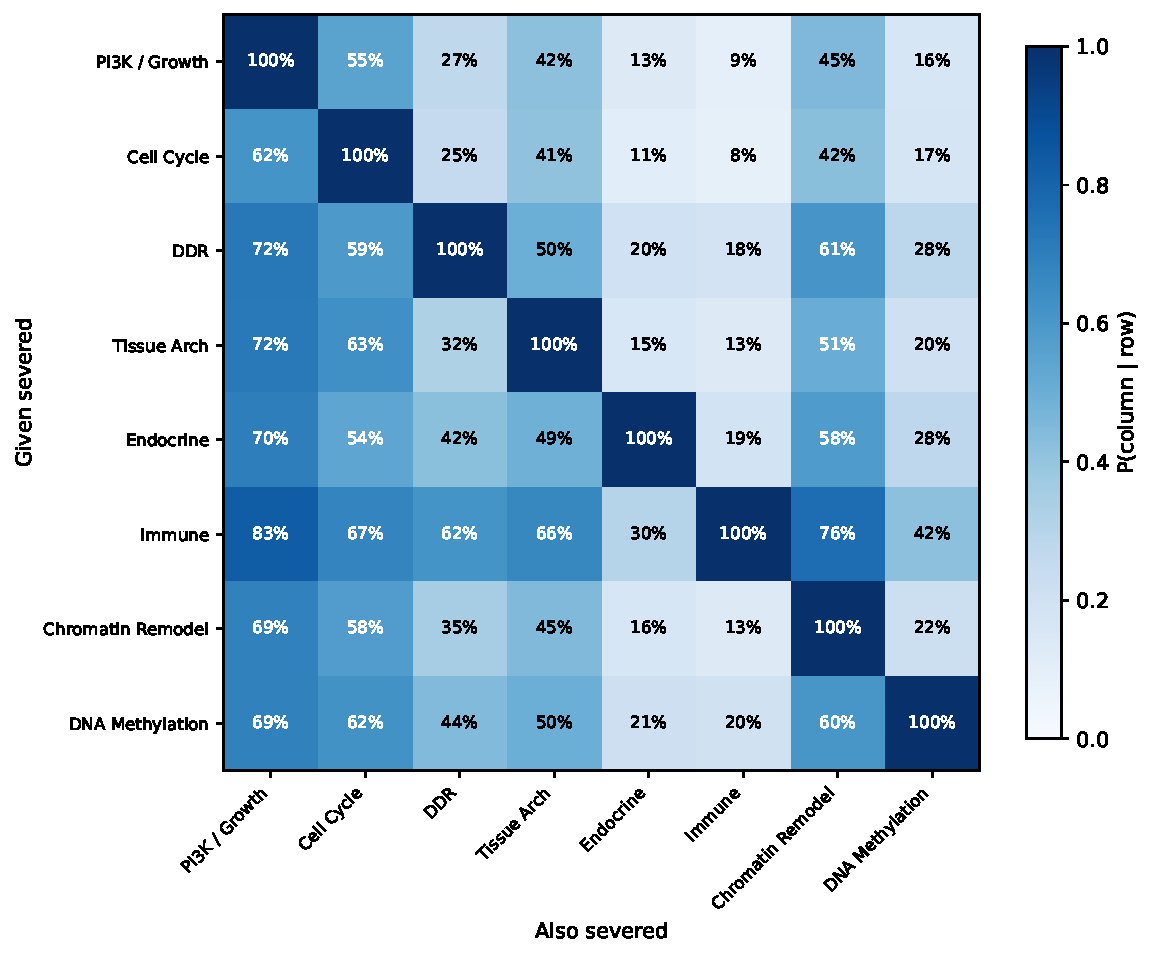
\includegraphics[width=0.7\textwidth]{channel_coseverance.pdf}
\caption{Channel co-severance matrix. Each cell shows
P(column channel severed $\mid$ row channel severed). The matrix is
asymmetric: cell-intrinsic channels (PI3K/Growth, Cell Cycle) predict
organism-level severance (Endocrine, Immune), but organism-level
severance does not predict cell-intrinsic. Severance propagates
inward toward the root of the escalation hierarchy.}
\label{fig:coseverance}
\end{figure}

The 1.9\% of multi-channel patients who lack a cell-intrinsic
gateway are enriched 6.5$\times$ for prostate, 2.5$\times$ for
breast, and 7.6$\times$ for mesothelioma: cancers entering through
organism level channels. Their lower mortality (34.8\% vs.\ 42.6\%)
is consistent: they have not escaped the most fundamental coupling
layer.

\textbf{The grouping must be biological, not statistical.}
Hierarchical clustering on Jaccard co-mutation distances ($k = 2$ to
$k = 10$) produces data-driven groupings that fail. At $k = 6$:
HR~$= 0.80$ ($p = 9 \times 10^{-6}$), the wrong direction.
Biological channels at $k = 6$: HR~$= 1.10$
($p = 3 \times 10^{-9}$). ARI between data-driven and biological
groupings: 0.018. Co-mutation clusters group genes by which tumors
they appear in. Channels group genes by which organizational system
they serve.

\textbf{Pathogenic variant restriction.} Restricting to truncating
mutations only, then truncating plus hotspot missense, the signal
strengthens: HR rises from 1.15 to 1.16 to 1.19
($p = 10^{-55}$). Mutation count becomes more protective
(HR~$= 0.75$ vs.\ 0.83 baseline). Removing VUS concentrates the
signal. The severance hierarchy is preserved.

\textbf{Panel bias.} MSK-IMPACT sequences 400--500 genes, a
fraction of the genome. Mutations in channel genes not on the panel
are undetected, systematically undercounting channel hits. This
compresses the channel-count gradient and works against the
hypothesis, not for it. The true association between channel count
and survival is likely stronger than what the panel captures.

\textbf{Limitations.} Stage at diagnosis and treatment history are
not available in these datasets. Channel count could correlate with
stage. Three partial controls mitigate this: (1) within-cancer-type
analysis, where stage distributions are more homogeneous;
(2) the 275-covariate model includes FGA and tumor purity, which
are stage-correlated proxies; (3) MetTropism is an all-metastatic
cohort where stage variation is minimal, and the signal replicates.
None of these fully substitute for stage adjustment. The analysis
also does not distinguish hub from leaf mutations within a channel.
The projection family predictions (Section~\ref{sec:predictions})
are untested.

% ------------------------------------------------------------------
\section{Structural Interpretation: Genome as Projection}
\label{sec:framework}
% ------------------------------------------------------------------

Mutations damage individual nodes. Channel damage destroys the
distributed connectivity between nodes. This section explains why.

\textbf{The projection forces three compromises.}
First, cycles must be broken. A linear sequence can only encode a
DAG. Feedback loops are severed during projection and reconstructed
at runtime via transcription factors, signaling cascades, and
chromatin looping. These reconstructed edges are the most fragile.

Second, hub nodes must be copied. A single address cannot serve all
adjacencies. The projection writes copies at different addresses.
What appears as genetic diversity is serialization overhead.

Third, distributed connectivity cannot be written at all. Channels
exist only in the three dimensional fold of the chromatin:
unprecipitated knowledge, reconstructed by physical proximity when
the helix folds.

\textbf{Bounded context and escalation.}
A cell can maintain a finite number of regulatory states ($C_n$)
\cite{Cowan2001}. Multicellular organization overcomes this through
hierarchical coupling: cell ($k\!=\!0$) escalates to tissue
($k\!=\!1$), organ ($k\!=\!2$), organism ($k\!=\!3$)
\cite{McCarthy2026c}. Coupling channels are the independent
dimensions of this hierarchy: gap junctions at the cell-tissue
boundary \cite{Aasen2016}, paracrine signaling at tissue-organ,
endocrine and immune at organ-organism \cite{Hanahan2011}.

\textbf{Chain severance.}
When a channel is lost, the cell's context contracts. Actions
requiring tissue level coordination become inaccessible
\cite{McCarthy2026a, McCarthy2026b}. What remains: proliferation,
metabolic autonomy, motility. Hanahan and Weinberg's hallmarks
\cite{Hanahan2011} are not acquired capabilities. They are the
convergent action space under cell level bounded context. The
Warburg effect is not a metabolic choice; it is the default when
tissue level information about oxygen supply is gone
\cite{Warburg1956}.

Each channel severed removes an independent class of coupling.
Mutation count measures depth within channels already severed;
deeper commitment to fewer escape routes produces a more
constrained tumor. The severance hierarchy (growth first, immune
last) is the escalation chain read in reverse: cell-tissue coupling
breaks before organism level coupling can be meaningfully exploited.

Two simultaneous channel breaks in one cell are lethal: the cell
loses two independent defense axes. Channel count at the patient
level therefore measures clonal diversity, not per-cell damage.
Multi-region sequencing confirms this architecture
\cite{Gerlinger2012, JamalHanjani2017}: trunk mutations (the
initiating channel break) are clonal; subsequent channel breaks
appear as subclonal branch events, with different tumor regions
independently converging on the same pathway through parallel
evolution. The tumor does not acquire new channels by choice. The
defense graph topology dictates which channel must break next; the
specific gene is stochastic.

\textbf{Projection families.}
Genes sharing interaction neighborhoods, mutation profiles, channel
assignments, and survival impact are projections of the same node.
The genome maintains redundant copies of critical subgraphs like a
RAID array. Lose one copy and the system degrades. Remove the parity
check (the synthetic lethal partner) and the degraded array fails.

Drug response follows projection families, not gene names. A PARP
inhibitor works regardless of which DDR copy is broken: BRCA1,
BRCA2, RAD51C, or any other projection of the same node. The drug
targets function, not address.

Chain severance occurs through multiple mechanisms: genetic, micro\-environmental,
epigenetic, spatial (Table~\ref{tab:severance-mechanisms}). All
produce the same outcome, explaining why hereditary, environmental,
and sporadic cancers converge on the same phenotypic endpoints.

% ------------------------------------------------------------------
\section{Predictions}
\label{sec:predictions}
% ------------------------------------------------------------------

Four classes of prediction follow from the projection framework:
expanded eligibility, combination futility, combination timing, and
untested targets.

\subsection{DDR family: PARP inhibitor eligibility expansion}

Current PARP inhibitor trials screen for a fixed list of DDR genes:
\emph{BRCA1}, \emph{BRCA2}, \emph{ATM}, \emph{PALB2},
\emph{RAD51C}, \emph{RAD51D}, \emph{FANCA}, \emph{FANCC},
\emph{FANCD2}. The framework predicts that additional DDR genes
sharing the same protein-protein interaction neighborhoods, mutation
type profiles, and survival impact should respond identically.
Candidates include \emph{BLM}, \emph{NBN}, \emph{ERCC4},
\emph{CHEK1}, \emph{CHEK2}, \emph{RAD51B}, \emph{RAD51},
\emph{BRIP1}, \emph{MRE11}, and \emph{XRCC2}. In the MSK-IMPACT
44{,}000-patient cohort, these genes collectively account for over
4{,}000 patients---nearly 10\% of the cohort---none of whom are
currently eligible for PARP inhibitor trials.

\textbf{Testable claim:} Patients with loss-of-function mutations in
\emph{BLM}, \emph{NBN}, \emph{ERCC4}, \emph{BRIP1}, or \emph{MRE11}
will show PARP inhibitor sensitivity comparable to \emph{BRCA2}
carriers, as measured by objective response rate and
progression-free survival.

\subsection{PI3K family: AKT/mTOR inhibitor eligibility expansion}

\emph{PIK3CA} and \emph{PTEN} respond to PI3K/AKT/mTOR inhibitors.
\emph{PIK3C2G}, \emph{INPP4B}, \emph{PIK3CB}, \emph{PIK3CD}, and
\emph{PIK3R3} are members of the same functional family with
overlapping interaction neighborhoods but no drug sensitivity data.

\textbf{Testable claim:} Loss-of-function mutations in
\emph{INPP4B}, \emph{PIK3CB}, and \emph{PIK3CD} confer sensitivity
to AKT inhibitors (e.g., capivasertib) comparable to
\emph{PTEN}-loss patients.

\subsection{FGF family: FGFR inhibitor eligibility expansion}

\emph{FGFR1}, \emph{FGFR2}, and \emph{FGFR3} respond to FGFR
inhibitors (erdafitinib, futibatinib). \emph{FGFR4} and
\emph{FGF4} are functional family members with no targeted
therapy data.

\textbf{Testable claim:} Activating mutations in \emph{FGFR4}
confer sensitivity to pan-FGFR inhibitors comparable to
\emph{FGFR2/3} fusion carriers.

\subsection{Chromatin remodeling: CREBBP/EP300}

\emph{CREBBP} and \emph{EP300} form one of the strongest functional
pairs in the model (3{,}491 combined patients). Both are histone
acetyltransferases with overlapping PPI neighborhoods and near-identical
mutation profiles. Neither has established targeted therapy.

\textbf{Testable claim:} \emph{CREBBP} and \emph{EP300} mutations
should respond to the same targeted therapy, once one exists. The
projection framework predicts functional equivalence; it does not
identify the drug. This is a prediction about family structure, not
a treatment recommendation.

\subsection{Same-channel combinations fail}

The framework predicts that combining two drugs targeting the same
coupling channel provides additive benefit at best, with compounding
toxicity. The second drug adds dose, not a new therapeutic axis.

\textbf{Testable claim:} PARP + ATR inhibitors, PARP + WEE1
inhibitors, PARP + ATM inhibitors, and dual PARP1/2 versus
PARP1-selective will show no significant PFS improvement over the
simpler regimen after adjusting for toxicity. Dual targeting within
a channel is architecturally redundant.

\subsection{Cross-channel combination timing}

Cross-channel combinations target two independent vulnerabilities.
The framework predicts they work only when \emph{both channels are
intact at treatment}.

\textbf{Metastatic futility:} In metastatic HR+ breast cancer
patients post-endocrine progression, adding a SERD (camizestrant)
to a PARP inhibitor (saruparib) will show minimal additional PFS
over PARP monotherapy. The endocrine escape has already occurred.

\textbf{Adjuvant harmonization:} In the adjuvant setting, low-dose
PARP1-selective inhibitor alongside endocrine therapy will produce
synergistic benefit in germline DDR carriers. The PARP kills cells
at DDR second-hit before they accumulate ESR1 resistance mutations.
The endocrine therapy maintains the channel those cells would have
escaped through. Each drug extends the other's efficacy.

Tamoxifen works adjuvantly because it maintains the endocrine
channel before severance. The same logic applies to DDR. PARP1-selective
inhibitors (saruparib) eliminate PARP2-driven hematological
suppression, enabling the long-term low-dose administration that
adjuvant use requires. OlympiA showed adjuvant olaparib is
tolerable alongside endocrine therapy; a PARP1-selective agent
should be more tolerable still.

\subsection{Testable observation: natural PARP1 disruption}

If projection families share drug vulnerability, then naturally
occurring \emph{PARP1} loss-of-function mutations should produce
the same synthetic lethality as PARP inhibitors in patients with
DDR partner mutations.

\textbf{Testable claim:} Patients with \emph{PARP1}
loss-of-function alongside DDR partner mutations will show improved
survival relative to DDR-mutant patients without \emph{PARP1}
mutations. A properly powered study with matched controls would
constitute a strong test of the synthetic lethality mechanism
independent of drug administration.

All drug-response predictions follow from one principle: screen by
functional node, not by gene name.

\subsection{Graph position predictions}

If projection families define which genes share a vulnerability,
graph position determines which phenotype results. Hub mutations
(high-connectivity, upstream) should produce worse outcomes and
broader phenotypes than leaf mutations (downstream, specific
effectors) in the same channel, because hubs sever more downstream
connections per event.

\textbf{Testable claim:} Hub mutations carry worse prognosis than
leaf mutations within the same channel, after controlling for
channel count and cancer type.

\textbf{Testable claim:} BRCA1 (DDR hub) and BRCA2 (DDR leaf)
produce divergent breast cancer phenotypes. BRCA1 mutations enrich
for triple-negative subtype and aggressive metastatic tropism.
BRCA2 mutations enrich for HR+ subtype and bone-predominant
metastasis. RAD51C, as a leaf-position DDR gene, phenocopies BRCA2,
not BRCA1.

Companion paper \cite{McCarthy2026f} tests these graph-position
predictions, including the distinction between gain-of-function
(which maintains coupling) and loss-of-function (which severs it),
and the directional escalation pattern within and across channels.

\subsection{Channel severance beyond genetics}

Channel severance occurs through any mechanism that disrupts the
coupling between organizational levels (Table~\ref{tab:severance-mechanisms}).
Genetic mutation is one route. Immunosuppression, neurodegeneration,
environmental disruption, and iatrogenic intervention are others.
If the framework is correct, non-genetic channel severance should
produce the same cancer risk predictions as genetic severance.

\textbf{Testable claim:} Organ transplant recipients on long-term
immunosuppression have artificially severed immune channels. The
framework predicts elevated cancer risk concentrated in immune-
surveillance-dependent cancer types, not uniform elevation across
all cancers. This is observed \cite{Engels2011}.

Non-genetic channel severance produces predictions spanning
psychiatry, neurology, and epidemiology. Companion paper
\cite{McCarthy2026h} develops these formally; here we note only that
the framework's logic applies to any severance mechanism, not
exclusively genetic mutation.

% ------------------------------------------------------------------
\section{Engagement with Prior Work}
\label{sec:prior}
% ------------------------------------------------------------------

Table~\ref{tab:prior-work} summarizes the relationship between
existing cancer frameworks and chain severance.

The closest existing framework is TOFT \cite{Sonnenschein2000}.
It correctly identifies the organizational level (tissue, not cell)
and the default proliferative state. Our framework provides the
formalism TOFT has lacked: the escalation chain is the formal
structure of tissue organization, $C_n^{\mathrm{eff}}$ is the
measure of organizational integration, and chain severance is
the formal description of organizational breakdown. TOFT's
``default proliferative state'' is our ``necessary action space
under cell level $C_n$.''

No existing cancer model addresses the projection layer. Current
frameworks treat genes as independent entities that participate in
shared pathways. The projection view treats them as copies of shared
functional nodes. This changes what it means to ``target a gene.''

% ------------------------------------------------------------------
\section{Conclusion}
\label{sec:conclusion}
% ------------------------------------------------------------------

Channel count predicts cancer survival ($p < 10^{-44}$). Mutation
count does not.

The structural interpretation: the genome is a linear projection
of a functional graph. Channels are the distributed connectivity
that no single gene encodes. Genes in the same projection family
carry the same drug vulnerability. Graph position within a family
determines phenotype. Channel severance by any mechanism, genetic
or otherwise, produces the same outcome.

This generates falsifiable predictions across four domains:
drug eligibility expansion (PARP, PI3K/AKT, FGFR), combination
therapy timing, graph position phenotyping, and non-genetic
channel severance (transplant immunosuppression, neurodegeneration,
information-environment cancer risk).

Screen by function, not by gene name. Companion papers test these
predictions \cite{McCarthy2026f, McCarthy2026h}. Formal derivations
appear in \cite{McCarthy2026a, McCarthy2026b, McCarthy2026c,
McCarthy2026d}.

\section*{Acknowledgments}

The author used Claude (Anthropic) for drafting assistance, literature review, and \LaTeX{} preparation. All theoretical content, proofs, and arguments are the author's own.

\bibliographystyle{plain}
\begin{thebibliography}{99}

\bibitem{Aasen2016}
T.~Aasen, M.~Mesnil, C.~C. Naus, P.~D. Lampe, and D.~W. Laird.
\newblock Gap junctions and cancer: Communicating for 50 years.
\newblock \emph{Nature Reviews Cancer}, 16(12):775--788, 2016.

\bibitem{Cowan2001}
N.~Cowan.
\newblock The magical number 4 in short-term memory: A reconsideration of
  mental storage capacity.
\newblock \emph{Behavioral and Brain Sciences}, 24(1):87--114, 2001.

\bibitem{Davies2011}
P.~C.~W. Davies and C.~H. Lineweaver.
\newblock Cancer tumors as {Metazoa} 1.0: Tapping genes of ancient ancestors.
\newblock \emph{Physical Biology}, 8(1):015001, 2011.

\bibitem{Hanahan2011}
D.~Hanahan and R.~A. Weinberg.
\newblock Hallmarks of cancer: The next generation.
\newblock \emph{Cell}, 144(5):646--674, 2011.

\bibitem{McCarthy2026a}
P.~D. McCarthy.
\newblock Graph structure is necessary for information preservation under
  bounded context.
\newblock Manuscript, 2026.

\bibitem{McCarthy2026b}
P.~D. McCarthy.
\newblock Knowledge as normalization: consistency under partition separates
  shared propositions from action.
\newblock Manuscript, 2026.

\bibitem{McCarthy2026c}
P.~D. McCarthy.
\newblock Convergence of control architectures to escalation under bounded context.
\newblock Manuscript, 2026.

\bibitem{McCarthy2026d}
P.~D. McCarthy.
\newblock Evaluation-driven descent, encoding permanence, and the structural
  invariants of intelligence.
\newblock Manuscript, 2026.

\bibitem{McCarthy2026f}
P.~D. McCarthy.
\newblock Mutation position in the signaling graph predicts cancer survival
  beyond channel count.
\newblock Manuscript, 2026.

\bibitem{Engels2011}
E.~A. Engels, R.~M. Pfeiffer, J.~F. Fraumeni, B.~L. Kasiske,
  A.~K. Israni, J.~J. Snyder, R.~A. Wolfe, N.~P. Goodrich,
  A.~L. Bayakly, G.~L. Clarke, and others.
\newblock Spectrum of cancer risk among {US} solid organ transplant
  recipients.
\newblock \emph{JAMA}, 306(17):1891--1901, 2011.

\bibitem{McCarthy2026h}
P.~D. McCarthy.
\newblock Context window diseases and cancer risk: Neural computation
  cost as a unifying mechanism.
\newblock Manuscript, 2026.

\bibitem{Sonnenschein2000}
C.~Sonnenschein and A.~M. Soto.
\newblock Somatic mutation theory of carcinogenesis: Why it should be dropped
  and replaced.
\newblock \emph{Molecular Carcinogenesis}, 29(4):205--211, 2000.

\bibitem{Vogelstein2013}
B.~Vogelstein, N.~Papadopoulos, V.~E. Velculescu, S.~Zhou, L.~A. Diaz, and
  K.~W. Kinzler.
\newblock Cancer genome landscapes.
\newblock \emph{Science}, 339(6127):1546--1558, 2013.

\bibitem{Warburg1956}
O.~Warburg.
\newblock On the origin of cancer cells.
\newblock \emph{Science}, 123(3191):309--314, 1956.

\bibitem{Cerami2012}
E.~Cerami, J.~Gao, U.~Dogrusoz, B.~E. Gross, S.~O. Sumer,
  B.~A. Aksoy, A.~Jacobsen, C.~J. Byrne, M.~L. Heuer,
  E.~Larsson, and others.
\newblock The {cBio} cancer genomics portal: An open platform for
  exploring multidimensional cancer genomics data.
\newblock \emph{Cancer Discovery}, 2(5):401--404, 2012.

\bibitem{Zehir2017}
A.~Zehir, R.~Benayed, R.~H. Shah, A.~Syed, S.~Middha,
  H.~R. Kim, P.~Srinivasan, J.~Gao, D.~Chakravarty,
  S.~M. Devlin, and others.
\newblock Mutational landscape of metastatic cancer revealed from
  prospective clinical sequencing of 10,000 patients.
\newblock \emph{Nature Medicine}, 23(6):703--713, 2017.

\bibitem{Nguyen2022}
B.~Nguyen, M.~G.~M. Fong, R.~K. Luthra, S.~M. Smith,
  R.~J. DiNatale, N.~Nandakumar, H.~Walch, W.~K. Chatila,
  R.~Madupuri, R.~Kundra, and others.
\newblock Genomic characterization of metastatic patterns from
  prospective clinical sequencing of 25,000 patients.
\newblock \emph{Cell}, 185(3):563--575, 2022.

\bibitem{Bandlamudi2024}
C.~Bandlamudi, J.~J.~Harding, A.~Zehir, and others.
\newblock Clinical genomic profiling of 50,000 patients:
  Experience from the {MSK-IMPACT} clinical sequencing cohort.
\newblock \emph{Cancer Cell}, 2026.

\bibitem{Gerlinger2012}
M.~Gerlinger, A.~J. Rowan, S.~Horswell, J.~Larkin, D.~Endesfelder,
  E.~Gronroos, P.~Martinez, N.~Matthews, A.~Stewart, P.~Tarpey, and others.
\newblock Intratumor heterogeneity and branched evolution revealed by
  multiregion sequencing.
\newblock \emph{New England Journal of Medicine}, 366(10):883--892, 2012.

\bibitem{JamalHanjani2017}
M.~Jamal-Hanjani, G.~A. Wilson, N.~McGranahan, N.~J. Birkbak,
  T.~B.~K. Watkins, S.~Veeriah, S.~Shafi, D.~H. Johnson,
  R.~Mitter, R.~Rosenthal, and others.
\newblock Tracking the evolution of non-small-cell lung cancer.
\newblock \emph{New England Journal of Medicine}, 376(22):2109--2121, 2017.

\bibitem{Swanton2023}
C.~Swanton, N.~McGranahan, G.~A. Wilson, and others (TRACERx Consortium).
\newblock The evolution of lung cancer and impact of subclonal selection
  in {TRACERx}.
\newblock \emph{Nature}, 616(7958):525--533, 2023.

\bibitem{Nowell1976}
P.~C. Nowell.
\newblock The clonal evolution of tumor cell populations.
\newblock \emph{Science}, 194(4260):23--28, 1976.

\bibitem{Huang2009}
S.~Huang, I.~Ernberg, and S.~Kauffman.
\newblock Cancer attractors: a systems view of tumors from a gene network
  dynamics and developmental perspective.
\newblock \emph{Seminars in Cell \& Developmental Biology}, 20(7):869--876,
  2009.

\bibitem{Aktipis2015}
C.~A. Aktipis, A.~M. Boddy, G.~Jansen, U.~Hibner, C.~C. Maley, and
  G.~S. Wilkinson.
\newblock Cancer across the tree of life: Cooperation and cheating in
  multicellularity.
\newblock \emph{Philosophical Transactions of the Royal Society B},
  370(1673):20140219, 2015.

\bibitem{Merlo2006}
L.~M.~F. Merlo, J.~W. Pepper, B.~J. Reid, and C.~C. Maley.
\newblock Cancer as an evolutionary and ecological process.
\newblock \emph{Nature Reviews Cancer}, 6(12):924--935, 2006.

\end{thebibliography}

\clearpage
\appendix
\section*{Tables}
\begin{landscape}

\begin{table}[p]
\centering
\caption{Mechanisms of chain severance. All four produce the same
outcome: $\lambda_j \to 0$, context collapse to $C_n^{(0)}$, and
cell-level optimization.}
\label{tab:severance-mechanisms}
\begin{tabular}{@{}llll@{}}
\toprule
Mechanism & How $\lambda_j \to 0$ & Example & Identified by \\
\midrule
Genetic & Cell's receivers damaged & E-cadherin loss, & SMT \\
 & & p53/Rb mutation & \cite{Vogelstein2013} \\[4pt]
Microenvironmental & Signal no longer & Chronic inflammation, & TOFT \\
 & transmitted & fibrosis, tissue damage & \cite{Sonnenschein2000} \\[4pt]
Epigenetic & Receiver genes silenced & Methylation of connexin & --- \\
 & without sequence change & or cadherin promoters & \\[4pt]
Spatial & Cell leaves & Basement membrane & --- \\
 & signaling field & breach, metastasis & \\
\bottomrule
\end{tabular}
\end{table}

\begin{table}[p]
\centering
\caption{Relationship to existing cancer frameworks.}
\label{tab:prior-work}
\begin{tabular}{@{}>{\raggedright}p{3.5cm}>{\raggedright}p{6cm}>{\raggedright\arraybackslash}p{12cm}@{}}
\toprule
Framework & What it captures & Our reinterpretation \\
\midrule
Hallmarks \cite{Hanahan2011}
 & Universal capabilities across cancers
 & Not acquired but \emph{revealed}: necessary action space under $C_n^{(0)}$ \\[4pt]
Atavistic theory \cite{Davies2011}
 & Phylostratigraphic gene pattern
 & Convergent necessity, not historical reversion \\[4pt]
Clonal evolution \cite{Nowell1976}
 & Darwinian selection dynamics
 & Provides the \emph{attractor}: direction is determined by $C_n^{(0)}$, not random \\[4pt]
Attractor landscape \cite{Huang2009}
 & Cancer as abnormal attractors
 & ``Abnormal'' attractors are the \emph{default} under cell-level $C_n$ \\[4pt]
Cancer as cheating \cite{Aktipis2015}
 & Cooperation breakdown
 & Cheating is not a strategy but the necessary outcome of chain severance \\[4pt]
Ecological process \cite{Merlo2006}
 & Tumor as ecosystem
 & Correct dynamics, but missing why they converge \\
\bottomrule
\end{tabular}
\end{table}

\begin{table}[p]
\centering
\caption{Complete gene-to-channel mapping used in all analyses.
Genes are assigned based on organizational function served, not
pathway membership alone. The full mapping (92 genes) and analysis
code are provided in the supplementary repository.}
\label{tab:gene-mapping}
\begin{tabular}{@{}>{\raggedright}p{4.5cm}>{\raggedright\arraybackslash}p{18cm}@{}}
\toprule
\textbf{Channel} & \textbf{Genes} \\
\midrule
DNA Damage Response &
  \emph{ATM}, \emph{ATR}, \emph{BRCA1}, \emph{BRCA2}, \emph{PALB2},
  \emph{RAD51C}, \emph{RAD51D}, \emph{RAD51B}, \emph{CHEK1},
  \emph{CHEK2}, \emph{BAP1}, \emph{BARD1}, \emph{FANCA},
  \emph{FANCC}, \emph{FANCD2}, \emph{MLH1}, \emph{MSH2},
  \emph{MSH6}, \emph{PMS2}, \emph{POLE}, \emph{POLD1} \\[6pt]
Cell Cycle / Apoptosis &
  \emph{TP53}, \emph{RB1}, \emph{CDKN1A}, \emph{CDKN1B},
  \emph{CDKN2A}, \emph{CDKN2B}, \emph{CDK4}, \emph{CDK6},
  \emph{CCND1}, \emph{CCNE1}, \emph{MDM2}, \emph{MDM4},
  \emph{MYC}, \emph{MYCN} \\[6pt]
PI3K / Growth Signaling &
  \emph{PIK3CA}, \emph{PIK3R1}, \emph{PTEN}, \emph{AKT1},
  \emph{AKT2}, \emph{AKT3}, \emph{MTOR}, \emph{KRAS}, \emph{NRAS},
  \emph{HRAS}, \emph{BRAF}, \emph{RAF1}, \emph{MAP2K1},
  \emph{MAP2K2}, \emph{MAP3K1}, \emph{MAP3K13}, \emph{ERBB2},
  \emph{ERBB3}, \emph{EGFR}, \emph{FGFR1}, \emph{FGFR2},
  \emph{FGFR3}, \emph{IGF1R}, \emph{MET}, \emph{NF1}, \emph{NF2},
  \emph{TSC1}, \emph{TSC2}, \emph{STK11}, \emph{ARID1A} \\[6pt]
Endocrine / Hormone &
  \emph{ESR1}, \emph{ESR2}, \emph{PGR}, \emph{AR}, \emph{FOXA1},
  \emph{GATA3} \\[6pt]
Immune Surveillance &
  \emph{B2M}, \emph{HLA-A}, \emph{HLA-B}, \emph{HLA-C},
  \emph{JAK1}, \emph{JAK2}, \emph{STAT1}, \emph{CD274},
  \emph{PDCD1LG2}, \emph{CTLA4} \\[6pt]
Tissue Architecture &
  \emph{CDH1}, \emph{CDH2}, \emph{CTNNB1}, \emph{APC},
  \emph{AXIN1}, \emph{AXIN2}, \emph{SMAD2}, \emph{SMAD3},
  \emph{SMAD4}, \emph{TGFBR1}, \emph{TGFBR2}, \emph{NOTCH1},
  \emph{NOTCH2}, \emph{NOTCH3}, \emph{NOTCH4}, \emph{FBXW7},
  \emph{GJA1}, \emph{GJB2} \\
\bottomrule
\end{tabular}
\end{table}

\end{landscape}

\end{document}
